\chapter{Experimentación}
\label{cap:experimentacion}

\section {Mapeado en entorno doméstico}
\label{cap:mapeadodomestico}

pruebas unitarias. CAMBIAR LAS IMAGENES DE DIRECTORIO


La figura \ref{fig:initserver} fue captada al iniciar el algoritmo. Observamos que la mayor parte del mapa de corto plazo se encuentra en una posición de desconocimiento y que se han ido incluyendo en este las zonas libres, las paredes y la estantería. Los puntos morados y verdes corresponden a la representación de las muestras tomadas por el láser.

\begin{figure}[H]
  \begin{center}
    \subfigure[]{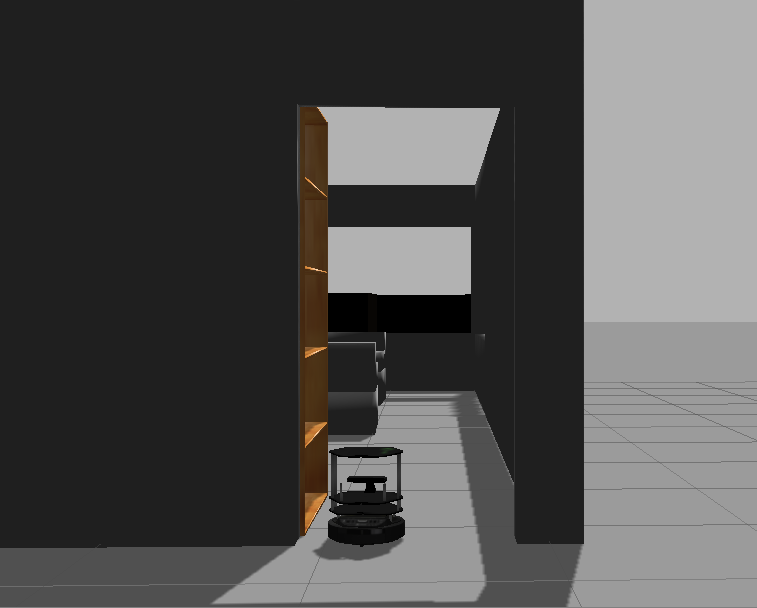
\includegraphics[width=5cm,height=5cm]{img/cap5/incrementmap}}
    \subfigure[]{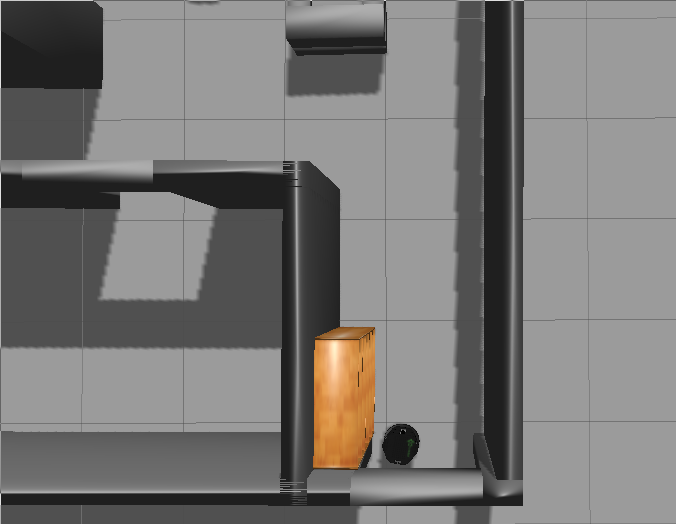
\includegraphics[width=5cm,height=5cm]{img/cap5/incrementmap2}}
    \subfigure[]{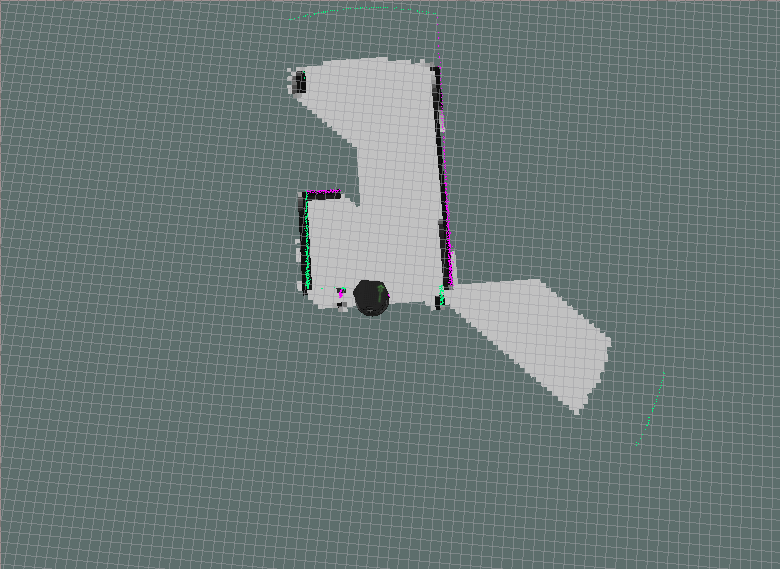
\includegraphics[width=5cm,height=5cm]{img/cap5/incrementmap-rviz}}
  \end{center}
  \caption{Visión del simulador, (a) y (b), y mapa a corto plazo (c).}
  \label{fig:initserver}
\end{figure}

Tras el inicio del algoritmo se añadió un objeto nuevo al escenario. Esto se representa en la figura \ref{fig:includeobject}. Vemos como el algoritmo añade el objeto al mapa y lo sitúa en una posición coherente respecto a la posición que ocupa el objeto en el escenario simulado.

\begin{figure} [H]
  \begin{center}
    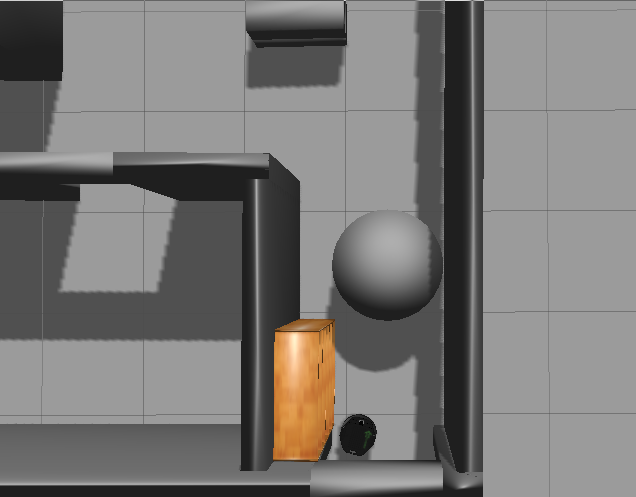
\includegraphics[width=6cm,height=5cm]{img/cap5/incrementmap-object3}
    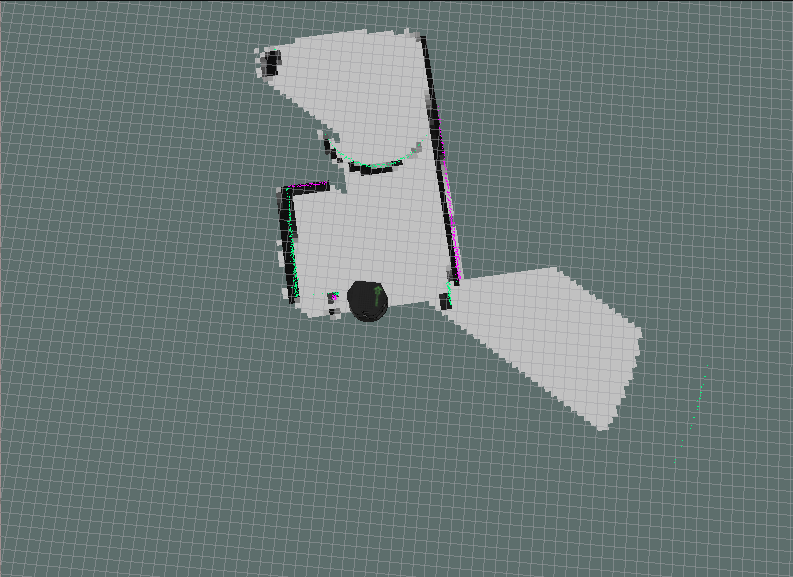
\includegraphics[width=6cm,height=5cm]{img/cap5/incrementmap-object}
  \end{center}
  \caption{Añadimos un objeto al escenario}
  \label{fig:includeobject}
\end{figure}

Una vez que el algoritmo a incluido el objeto en el mapa procedemos a eliminarlo del escenario simulado. Esto se representa en la figura  \ref{fig:deleteobject}. Vemos como el algoritmo ha comenzado a borrar el objeto, por lo que el valor de las celdas que estaban ocupadas por el objeto ahora es mucho menor.

\begin{figure}[H]
  \begin{center}
    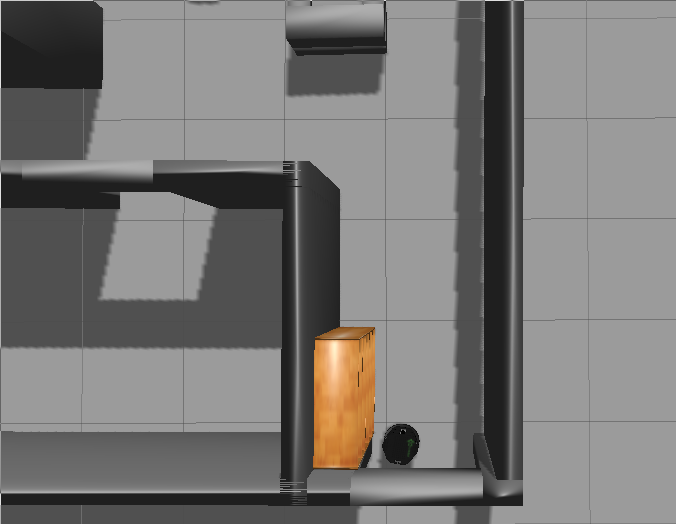
\includegraphics[width=6cm,height=5cm]{img/cap5/incrementmap2}
    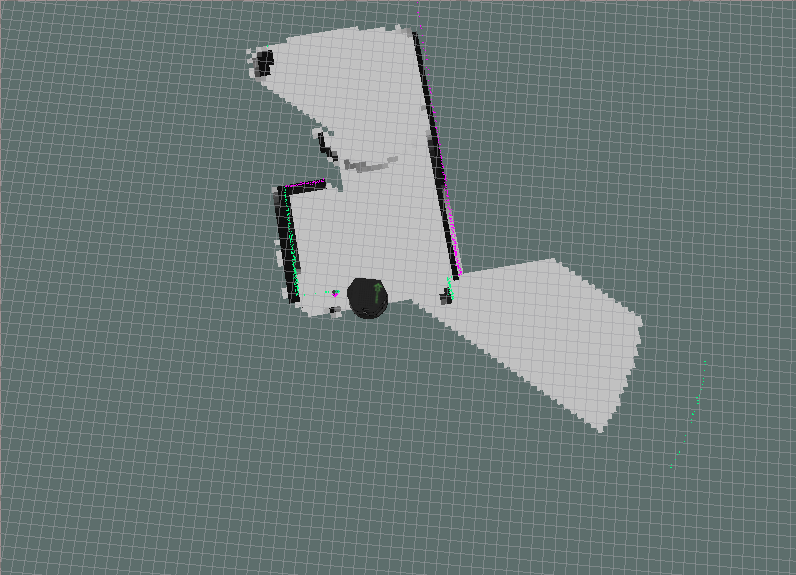
\includegraphics[width=6cm,height=5cm]{img/cap5/incrementmap-object2}
  \end{center}
  \caption{Eliminamos un objeto del escenario}
  \label{fig:deleteobject}
\end{figure}

\section {Navegación con obstáculos dinámicos}
\label{cap:navegacionconobstaculos}

\section {Experimentación en la Robocup}
\label{cap:experimentacionrobocup}




LARGO PLAZO

\begin{figure}[H]
  \begin{center}
    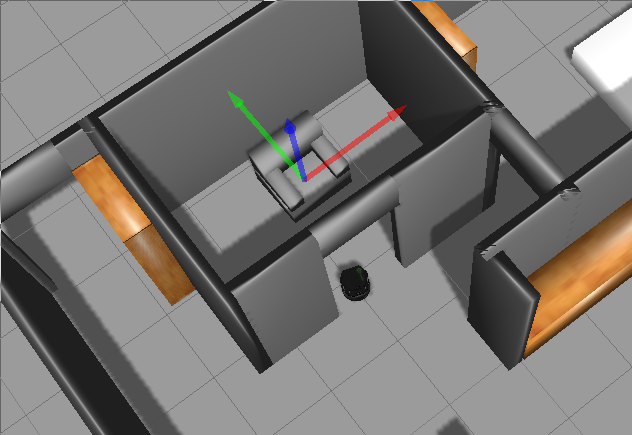
\includegraphics[width=10cm,height=6cm]{img/cap5/addingobject-gazebo}
    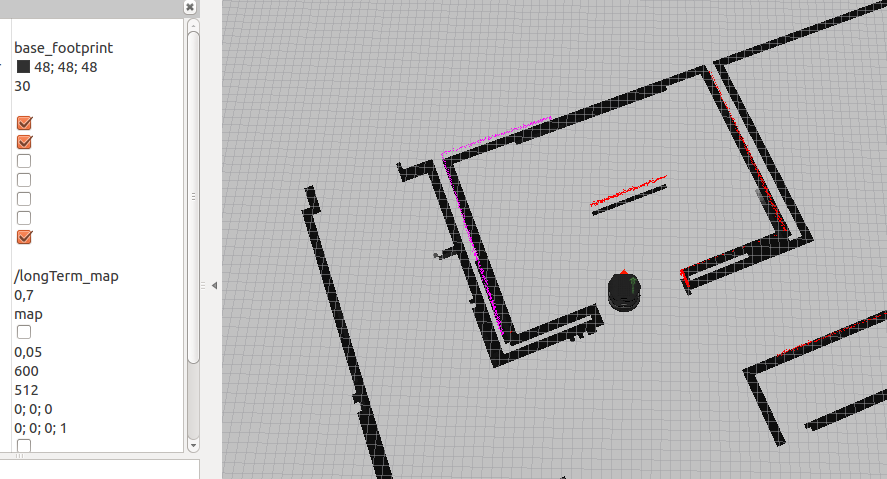
\includegraphics[width=10cm,height=5cm]{img/cap5/addingobject-longmap}
  \end{center}
  \caption{Añadimos un objeto al mapa de largo plazo}
  \label{fig:addobjectlongmap}
\end{figure}

\begin{figure}[H]
  \begin{center}
    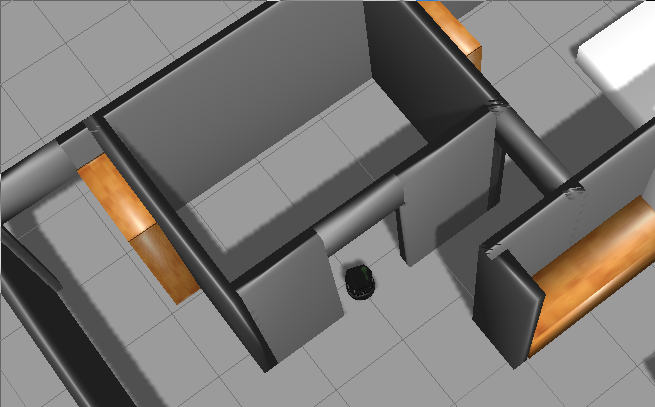
\includegraphics[width=10cm,height=5cm]{img/cap5/deletingobject-gazebo}
    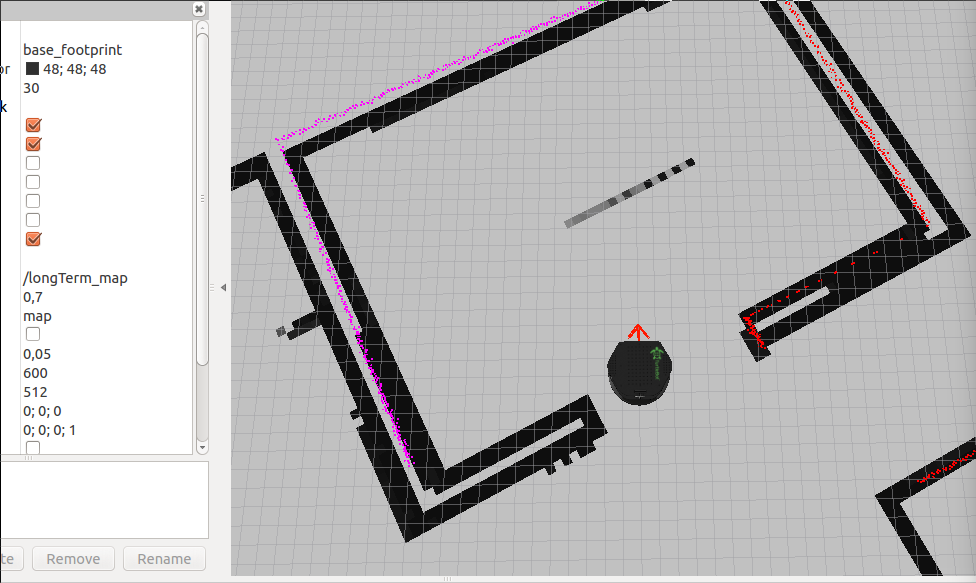
\includegraphics[width=10cm,height=5cm]{img/cap5/deletingobject-longmap}
  \end{center}
  \caption{Borramos un objeto del mapa de largo plazo}
  \label{fig:deleteobjectlongmap}
\end{figure}




{Navegacion por entornos desconocidos}

Además esta modificación nos ha permitido localizarnos en entornos desconocidos, es decir, ahora contamos con la capacidad de navegar por estancias de una casa que no tenemos en el mapa. Estas estancias se irán añadiendo al mapa de corto plazo primero y más tarde al mapa de largo plazo y el algoritmo de localización puede seguir calculando nuestra posición en los nuevos mapas.

\begin{figure}[hbtp]
  \begin{center}
    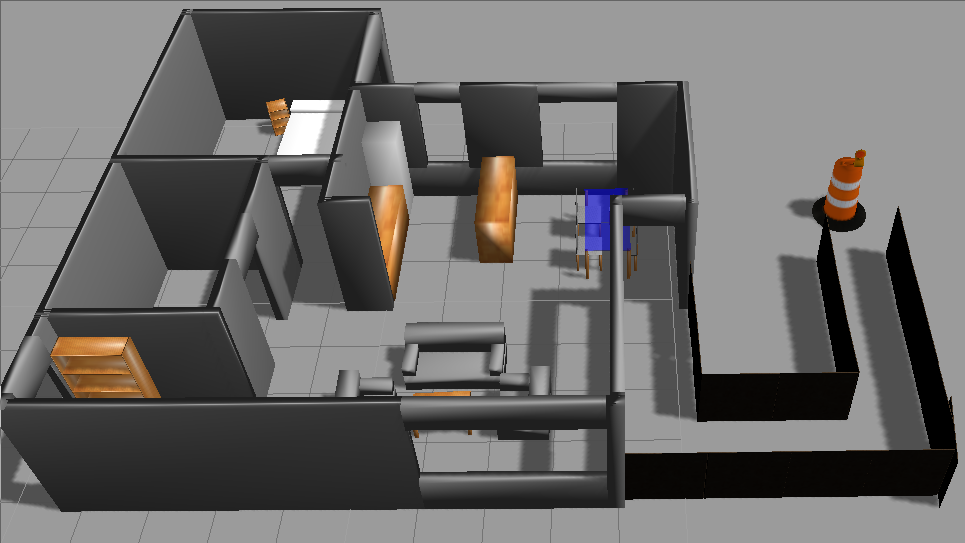
\includegraphics[width=12cm,height=7cm]{img/cap7/grannieAnne-ext}
  \end{center}
  \caption{Escenario extendido}
  \label{fig:grannieAnne-ext}
\end{figure}

\begin{figure}[hbtp]
  \begin{center}
    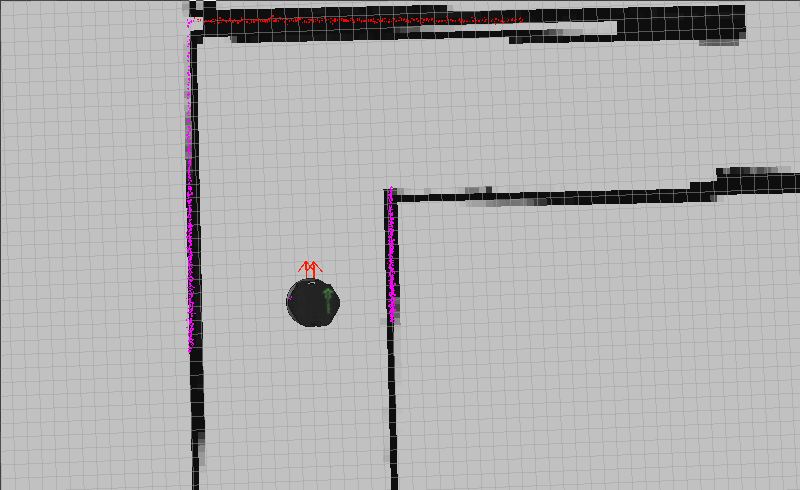
\includegraphics[width=10cm,height=6cm]{img/cap7/localization-ext}
  \end{center}
  \caption{Detalle de la localización}
  \label{fig:localization-ext}
\end{figure}


\begin{figure}[hbtp]
  \begin{center}
    \subfigure[Mapa total]{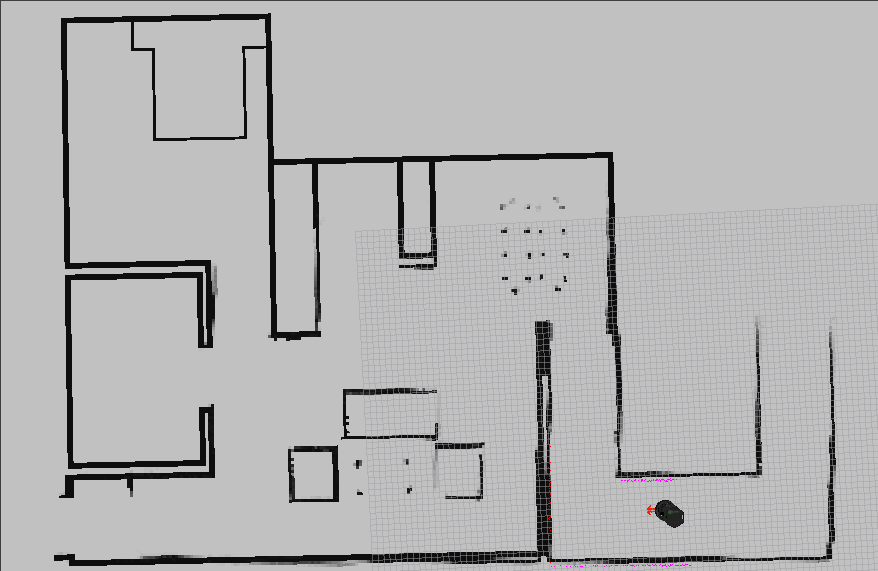
\includegraphics[width=12cm,height=7cm]{img/cap7/map-ext}}
    \subfigure[Mapa de largo plazo]{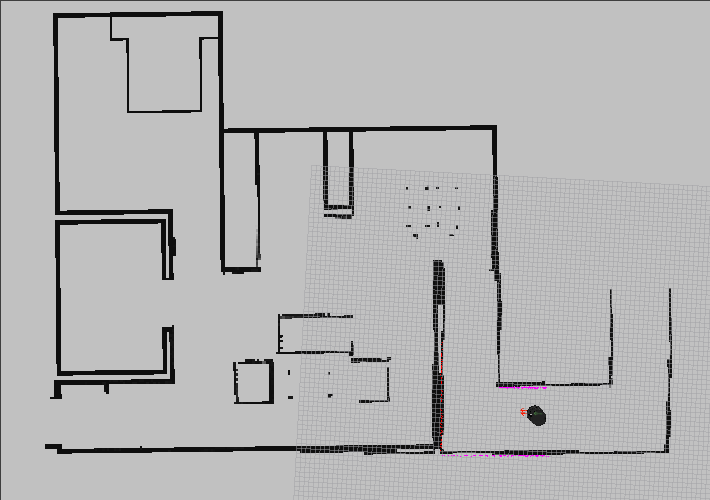
\includegraphics[width=12cm,height=7cm]{img/cap7/longmap-ext}}
    \subfigure[Mapa de corto plazo]{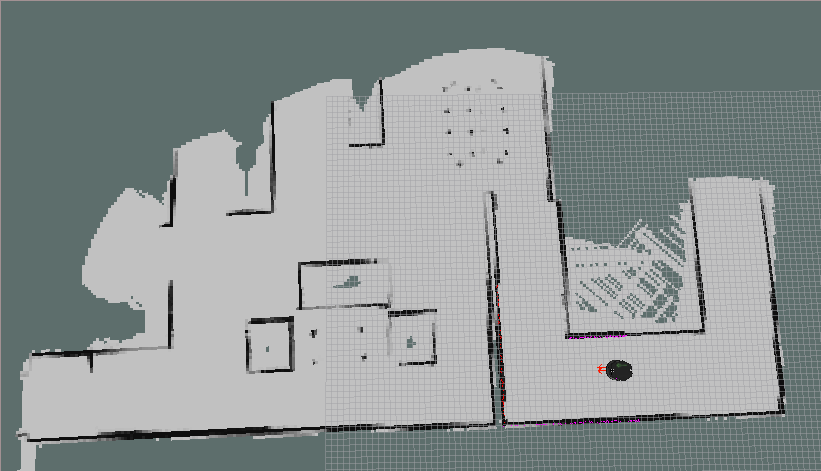
\includegraphics[width=12cm,height=7cm]{img/cap7/shortmap-ext}}
  \end{center}
  \caption{Mapas del escenario extendido}
  \label{fig:maps-ext}
\end{figure}

En la figura \ref{fig:grannieAnne-ext} vemos como el escenario ha sido extendido, añadiéndole unos pasillos a la derecha de la casa. El mapa estático usado es el mismo que el mostrado en la figura \ref{fig:mapaestatico}. Vemos como después de recorrer la parte desconocida del mapa se ha añadido al mapa de largo plazo y también al mapa total, figura \ref{fig:maps-ext}. Observamos en las flechas rojas bajo el robot que la incertidumbre en la posición del robot es mínima, figura \ref{fig:localization-ext}. 